\documentclass[10pt,a4paper]{amsart}
\usepackage[margin=19mm]{geometry}
\usepackage{amsmath,amssymb,mathtools}
\usepackage[scr=rsfs,cal=euler]{mathalfa}
\usepackage{xfrac}
\usepackage[unicode,hidelinks,bookmarks=false]{hyperref}
\newcommand{\ie}{i.e.\ }
\newcommand{\cf}{cf.\ }
\newcommand{\resp}{respectively\ }
\newcommand{\Subsection}{\subsection}
\providecommand{\nobreakdash}{\nobreak\hbox{-}}
\setlength{\emergencystretch}{2em}
\multlinegap0pt
\usepackage{tikz}
\newtheorem{theorem}{Theorem}
\title{Average Steps Until Absorption on Random Walks on Sea Dragon Trees}
\author{John Estes*}
\date{Source: arXiv:2604.23379v1 (CC BY 4.0)}
\begin{document}
\maketitle

\noindent\emph{Source and licence.} Average Steps Until Absorption on Random Walks on Sea Dragon Trees. Version arXiv:2604.23379v1 (CC BY 4.0), distributed by arXiv under the Creative Commons Attribution 4.0 International licence, http://creativecommons.org/licenses/by/4.0/, as recorded in the arXiv licence metadata for this exact version and shown on the abstract page https://arxiv.org/abs/2604.23379v1. Full licence notice: \texttt{licenses/arxiv-2604.23379-CC-BY-4.0.txt}.\par\smallskip

\noindent\textit{Editorial scope.} Counted unit: the article's theorem thm:sd1 (source0.tex lines 1238--1249). The article's complete original proof of it is delivered with it (source0.tex lines 1251--1517, one \texttt{proof} environment of 267 lines). No mathematics is written, repaired or re-derived: the statement and the proof are the article's own lines, in the article's own notation, and no retained line is substituted or re-flowed.  No further source-local context is needed: every cross-reference of every retained line resolves inside the two delivered spans.  Nothing was omitted from any retained span, so the package carries no omission record.  No retained line contains a citation, so the wrapper carries no bibliography and no bibliography entry.  The retained lines contain the article's own diagram code, which the wrapper typesets with the standard tikz packages; no image file is delivered and the package declares no asset dependency.  Editorial formatting only, in addition: an AMS \texttt{amsart} preamble that restates the article's own declarations and macros used by the retained lines, namely the environments \texttt{theorem} on separate counters, together with the standard packages those lines need.  The retained environments print in this document as Theorem 1 in order of appearance, whereas the article prints the same items with the numbering of its own full document.  The complete native source of the article as distributed in the arXiv e-print for this exact version is bundled unchanged as \texttt{sources/199160/source0.tex}.
\begin{theorem}[ASUAs of SD1 Trees]
\label{thm:sd1}
\noindent Let $G = T(n,\{k_1,\ldots, k_a\})$, $t(v_i) = t(G,v_i,v_n)$, and, by convention, $k_0 = 1$. Then for $0 \leq s \leq a-1$,

\[
t(v_i) = 
\begin{cases}
    n^2- i^2 +2(a-1)n -2(s-1)i -2\displaystyle\sum_{j=s+1}^a k_j, & \text{for } k_s \leq i \leq k_{s+1} \\
    n^2- i^2 + 2(a-1)(n-i), & \text{for } k_{a} \leq i \leq n-1 
\end{cases}
\]
\end{theorem}

\begin{proof}

\noindent Let $g(s,i) = n^2- i^2 +2(a-1)n -2(s-1)i -2\sum_{j=s+1}^a k_j, \text{ for } k_s \leq i \leq k_{s+1}$ and $g(a,i)=  n^2- i^2 + 2(a-1)(n-i), \text{ for } k_{a} \leq i \leq n-1$. Note that if we allow $\sum_{j=a+1}^a k_j$ to take the value of 0, then $g(s,i) = n^2- i^2 +2(a-1)n -2(s-1)i -2\sum_{j=s+1}^a k_j$ for all values of $i$ and $s$. To help communicate structure needed in our argument, we say vertices \{$v_{k_s}, v_{k_s + 1}, \ldots, v_{k_{s+1} -1}$\} form a \emph{section} of the graph.

\noindent We will show that $g(s,i)$ is consistent solution to ASUA equations associated with the graph in all cases. We first look at the end cases of $i=1$ and $i = n-1$.

\noindent Let $i=1$ and $k_1 > 2$. Then $t(v_1)  = t(v_2) + 1 = g(0,2) + 1 = n^2 - 1^2 + 2(a-1)n + 2 - 2\sum_{j = 1}^a k_j = g(0,1)$. Likewise if $k_1 = 2$, then $t(v_2) + 1 = g(1,2) + 1 = n^2 - 1^2 - 3 + 2(a-1)n - 0 - 2\sum_{j = 1}^a k_j + 1 = n^2 - 1^2 - 2(a-1)n - 2(0-1) - 2\sum_{j = 1}^a k_j = g(0,1)$.

\noindent Now let $i = n-1$ and $k_a < n-1$. Then $t(v_{n-1}) = \dfrac{1}{2}t(v_{n-2}) + 1 = \dfrac{1}{2}g(a, n-2) + 1$. Thus

\begin{align*}
    t(v_{n-1}) & = \dfrac{1}{2}(n^2 - (n-2)^2 + 2(a-1)n - 2(a-1)(n-2)) + 1 \\
    & = \dfrac{1}{2}(4n - 4 + 2(a-1)(n - (n-2))) + 1 \\
    & = 2n -2 + 2(a-1) + 1 \\
    & = n^2 - n^2 + 2n -1 + 2(a-1)(n-(n-1)) = g(a,n-1).
\end{align*}

If $k_a = n-1$. Thus $t(v_{n-1}) = \dfrac{1}{2}t(v_{n-2}) + 2 = \dfrac{1}{2}g(a-1, n-2) + 2$, and so

\begin{align*}
    t(v_{n-1}) & = \dfrac{1}{2}(n^2 - (n-2)^2 + 2(a-1)n - 2(a-2)(n-2) - 2k_a) + 2 \\
    & = 2n -2 + (a-1)n - (a-2)(n-2) - (n-1) + 2 \\
    & = n^2 - (n-1)^2 + 2a - 4 + 2 \\
    & = n^2 - (n-1)^2 + 2(a-1) = g(a,n-1).
\end{align*}

\noindent We now turn to $t(v_i)$ for $2 \leq i \leq n-2$. The local structure of $v_{i-1}, v_i,$ and $v_{i+1}$ falls into one of four types pictured in Figure \ref{tikz_sd1proof}. 


\begin{figure}[h] 
\label{tikz_sd1proof}
\begin{center}
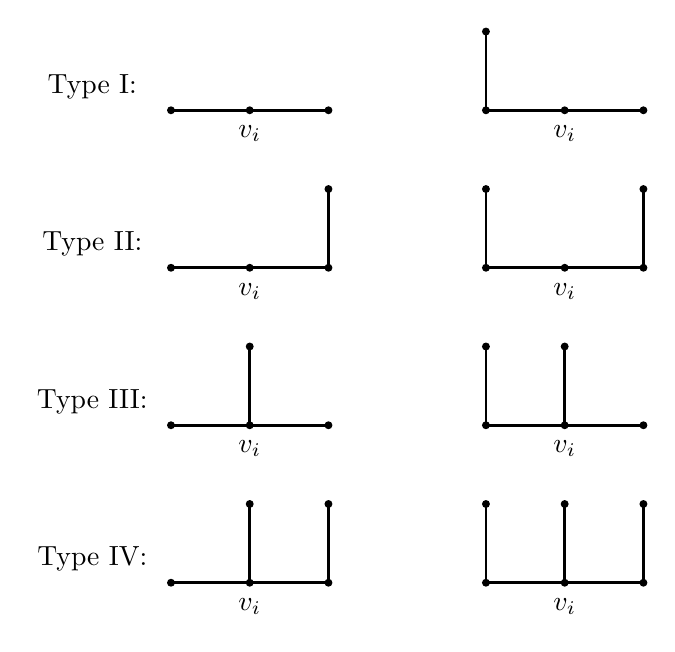
\begin{tikzpicture}[scale=1]
%------------------ TYPE I---------------------
\coordinate (A) at (-3,4);
\coordinate (B) at (-2,4);
\coordinate (C) at (-1,4);
\coordinate (D) at (0,4);
\coordinate (E) at (1,4);
\coordinate (F) at (2,4);
\coordinate (G) at (3,4);

%\coordinate (H) at (-2,5);
\coordinate (I) at (1,5);
\coordinate (J) at (3,5);

\draw [fill=black,thick] (A) circle [radius=1pt];
\draw [fill=black,thick] (B) circle [radius=1pt];
\draw [fill=black,thick] (C) circle [radius=1pt];
%\draw [fill=black,thick] (D) circle [radius=1pt];
\draw [fill=black,thick] (E) circle [radius=1pt];
\draw [fill=black,thick] (F) circle [radius=1pt];
\draw [fill=black,thick] (G) circle [radius=1pt];
%\draw [fill=black,thick] (H) circle [radius=1pt];
\draw [fill=black,thick] (I) circle [radius=1pt];
%\draw [fill=black,thick] (J) circle [radius=1pt];

\draw [line width=1pt] (A) to (B);
\draw [line width=1pt] (B) to (C);

%\draw [line width=1pt] (D) to (E);
\draw [line width=1pt] (E) to (F);
\draw [line width=1pt] (F) to (G);
%\draw [line width=1pt] (B) to (H);
\draw [line width=1pt] (E) to (I);
%\draw [line width=1pt] (G) to (J);

\node at (-4,4.3) {Type I:};
\node at (-2,3.7) {$v_i$};
\node at (2,3.7) {$v_i$};

%-------------TYPE II--------------------------

\coordinate (A1) at (-3,2);
\coordinate (B1) at (-2,2);
\coordinate (C1) at (-1,2);
\coordinate (D1) at (0,2);
\coordinate (E1) at (1,2);
\coordinate (F1) at (2,2);
\coordinate (G1) at (3,2);
%\coordinate (H1) at (4,2);
%\coordinate (I1) at (5,2);
%\coordinate (J1) at (6,2);
%\coordinate (K1) at (7,2);

\coordinate (L1) at (-1,3);
\coordinate (M1) at (1,3);
\coordinate (N1) at (3,3);
%\coordinate (O1) at (5,3);
%\coordinate (P1) at (6,3);
%\coordinate (Q1) at (7,3);

\draw [fill=black,thick] (A1) circle [radius=1pt];
\draw [fill=black,thick] (B1) circle [radius=1pt];
\draw [fill=black,thick] (C1) circle [radius=1pt];
%\draw [fill=black,thick] (D) circle [radius=1pt];
\draw [fill=black,thick] (E1) circle [radius=1pt];
\draw [fill=black,thick] (F1) circle [radius=1pt];
\draw [fill=black,thick] (G1) circle [radius=1pt];
%\draw [fill=black,thick] (H1) circle [radius=1pt];
%\draw [fill=black,thick] (I1) circle [radius=1pt];
%\draw [fill=black,thick] (J1) circle [radius=1pt];
%\draw [fill=black,thick] (K1) circle [radius=1pt];

\draw [fill=black,thick] (L1) circle [radius=1pt];
\draw [fill=black,thick] (M1) circle [radius=1pt];
\draw [fill=black,thick] (N1) circle [radius=1pt];
%\draw [fill=black,thick] (O1) circle [radius=1pt];
%\draw [fill=black,thick] (P1) circle [radius=1pt];
%\draw [fill=black,thick] (Q1) circle [radius=1pt];

\draw [line width=1pt] (A1) to (B1);
\draw [line width=1pt] (B1) to (C1);
\draw [line width=1pt] (E1) to (F1);
\draw [line width=1pt] (F1) to (G1);
%\draw [line width=1pt] (I1) to (J1);
%\draw [line width=1pt] (J1) to (K1);


\draw [line width=1pt] (C1) to (L1);
\draw [line width=1pt] (E1) to (M1);
\draw [line width=1pt] (G1) to (N1);
%\draw [line width=1pt] (I1) to (O1);
%\draw [line width=1pt] (J1) to (P1);
%\draw [line width=1pt] (K1) to (Q1);

\node at (-4,2.3) {Type II:};
\node at (-2,1.7) {$v_i$};
\node at (2,1.7) {$v_i$};


%-------------TYPE III--------------------------

\coordinate (A2) at (-3,0);
\coordinate (B2) at (-2,0);
\coordinate (C2) at (-1,0);
\coordinate (D2) at (0,0);
\coordinate (E2) at (1,0);
\coordinate (F2) at (2,0);
\coordinate (G2) at (3,0);
\coordinate (H2) at (4,0);


 \coordinate (I2) at (-2,1); 
% \coordinate (K2) at (7,0);
\coordinate (L2) at (1,1);
\coordinate (J2) at (2,1);

\draw [fill=black,thick] (A2) circle [radius=1pt];
\draw [fill=black,thick] (B2) circle [radius=1pt];
\draw [fill=black,thick] (C2) circle [radius=1pt];
%\draw [fill=black,thick] (D) circle [radius=1pt];
\draw [fill=black,thick] (E2) circle [radius=1pt];
\draw [fill=black,thick] (F2) circle [radius=1pt];
\draw [fill=black,thick] (G2) circle [radius=1pt];
%\draw [fill=black,thick] (H) circle [radius=1pt];

\draw [fill=black,thick] (L2) circle [radius=1pt];
\draw [fill=black,thick] (I2) circle [radius=1pt];
\draw [fill=black,thick] (J2) circle [radius=1pt];

\draw [line width=1pt] (A2) to (B2);
\draw [line width=1pt] (B2) to (C2);
\draw [line width=1pt] (E2) to (F2);
\draw [line width=1pt] (F2) to (G2);
\draw [line width=1pt] (L2) to (E2);
\draw [line width=1pt] (I2) to (B2);
\draw [line width=1pt] (J2) to (F2);

\node at (-4,.3) {Type III:};
\node at (-2,-.3) {$v_i$};
\node at (2,-.3) {$v_i$};

%-------------TYPE IV--------------------------

\coordinate (A3) at (-3,-2);
\coordinate (B3) at (-2,-2);
\coordinate (C3) at (-1,-2);
\coordinate (D3) at (-2,-1);
\coordinate (E3) at (-1,-1);
\coordinate (F3) at (-1,-2);
\coordinate (H3) at (0,-2);
\coordinate (I3) at (1,-2);
\coordinate (J3) at (2,-2);
\coordinate (K3) at (3,-2);
\coordinate (L3) at (1,-1);
\coordinate (M3) at (2,-1);
\coordinate (N3) at (3,-1);


\draw [fill=black,thick] (A3) circle [radius=1pt];
\draw [fill=black,thick] (B3) circle [radius=1pt];
\draw [fill=black,thick] (C3) circle [radius=1pt];
\draw [fill=black,thick] (D3) circle [radius=1pt];
\draw [fill=black,thick] (E3) circle [radius=1pt];
\draw [fill=black,thick] (I3) circle [radius=1pt];
\draw [fill=black,thick] (J3) circle [radius=1pt];
\draw [fill=black,thick] (K3) circle [radius=1pt];
\draw [fill=black,thick] (L3) circle [radius=1pt];
\draw [fill=black,thick] (M3) circle [radius=1pt];
\draw [fill=black,thick] (N3) circle [radius=1pt];

\draw [line width=1pt] (A3) to (B3);
\draw [line width=1pt] (B3) to (C3);
\draw [line width=1pt] (D3) to (B3);
\draw [line width=1pt] (E3) to (C3);
\draw [line width=1pt] (I3) to (J3);
\draw [line width=1pt] (J3) to (K3);
\draw [line width=1pt] (I3) to (L3);
\draw [line width=1pt] (J3) to (M3);
\draw [line width=1pt] (K3) to (N3);

\node at (-4,-1.7) {Type IV:};
\node at (-2,-2.3) {$v_i$};
\node at (2,-2.3) {$v_i$};

\end{tikzpicture}
\end{center}
\caption{Structure types for SD1}
\label{grotlem2}
\end{figure}


\noindent The Type I structure is characterized by $v_{i-1}, v_i,$ and $v_{i+1}$ all belonging to the same section. In this case, $t(v_i) = \dfrac{1}{2}(g(s,i-1) + g(s,i+1)) + 1$. Thus

\begin{align*}
    t(v_i) & = \dfrac{1}{2}(g(s,i-1) + g(s,i+1)) + 1 \\
          & = n^2 + 2(a-1)n - 2\displaystyle \sum_{j = s+1}^a k_j - (i^2 + 1) \\
            & \hspace{.5in} + \dfrac{1}{2}(-2(s-1)(i - 1) - 2(s-1)(i+1)) + 1 \\
            & = n^2 - i^2 - 2(a-1)n - 2(s-1)i - 2\displaystyle \sum_{j = s+1}^a k_j - 1 + 1\\
            & = g(s,i).
\end{align*}

\noindent Type II structure is characterized by $v_{i-1}$ and $v_i$ belonging to the $s^{th}$ section while $v_{i+1}$ in the $(s+1)^{th}$ section. In this case, $v_i = k_{s+1} - 1$ and $t(v_i) = \dfrac{1}{2}(g(s,i-1) + g(s,i+1)) + 1$. Thus,

\begin{align*}
    t(v_i) & = \dfrac{1}{2}(g(s,i-1) + g(s+1,i+1)) + 1 \\
          & = n^2 + 2(a-1)n - i^2 -1 \, +  \\
            & \hspace{.5in} + \dfrac{1}{2}(-2(s-1)(i - 1) - 2s(i+1) - 2\displaystyle \sum_{j = s+1}^a k_j - 2\displaystyle \sum_{j = s+2}^a k_j) + 1 \\
            & = n^2 - i^2 - 2(a-1)n - 2si + 2i - i - 1- 2\displaystyle \sum_{j = s+2}^a k_j - k_{s+1} \\
            & = n^2 - i^2 - 2(a-1)n - 2(s-1)i - k_{s+1} + 1 -1 -  2\displaystyle \sum_{j = s+2}^a k_j - k_{s+1} \\
            & = g(s,i).
\end{align*}

\noindent Type III structure is characterized by $v_{i-1}$ belonging to the $(s+1)^{th}$ section while $v_i$ and $v_{i+1}$ belong to the $s^{th}$ section. In this case, $v_i = k_{s}$ and $t(v_i) = \dfrac{1}{2}(g(s-1,i-1) + g(s,i+1)) + 2$. Thus,

\begin{align*}
    t(v_i) & = \dfrac{1}{2}(g(s-1,i-1) + g(s,i+1)) + 2 \\
          & = n^2 + 2(a-1)n - i^2 -1 \, +  \\
            & \hspace{.5in} + \dfrac{1}{2}(-2(s-2)(i - 1) - 2(s-1)(i+1) - 2\displaystyle \sum_{j = s}^a k_j - 2\displaystyle \sum_{j = s+1}^a k_j) + 2 \\
            & = n^2 - i^2 - 2(a-1)n - 1 - 2si + 2i + i - 1- 2\displaystyle \sum_{j = s+1}^a k_j - k_{s} + 2 \\
            & = g(s,i) -2 + k_s - k_s + 2 = g(s,i).
\end{align*}

\noindent Lastly, Type IV structure is characterized by each of $v_{i-1}, v_i$, and $v_{i+1}$ all belonging to different sections. In this case, $i = k_s = k_{s+1} -1$, and $t(v_i) = \dfrac{1}{2}(g(s-1,i-1) + g(s+1,i+1)) + 2$. Thus,

\begin{align*}
    t(v_i) & = \dfrac{1}{2}(g(s-1,i-1) + g(s+1,i+1)) + 2 \\
          & = n^2 + 2(a-1)n - i^2 -1 \, +  \\
            & \hspace{.5in} + \dfrac{1}{2}(-2(s-2)(i - 1) - 2s(i+1) - 2\displaystyle \sum_{j = s}^a k_j - 2\displaystyle \sum_{j = s+s}^a k_j) + 2 \\
            & = n^2 - i^2 - 2(a-1)n - 1 - 2si + 2i + 2 - 2\displaystyle \sum_{j = s+1}^a k_j - k_{s} - (k_{s} + 1) + 2 \\
            & = g(s,i) - 1 + k_s - k_s -1 + 2 = g(s,i).
\end{align*}

\noindent Thus $t(v_i) = g(s,i)$ for all values of $i$ proving the theorem.

\end{proof}

\end{document}
